\chapter{Practical guide to \enquote{ClassicThesis at DEIB}}
\label{chap:conclusion}
This template is ready to be used when writing a thesis at \myDepartment.
It is a modified version of Classic Thesis by Andr\'e Miede that can be found here \url{http://code.google.com/p/classicthesis/}.

\section{Learn \LaTeX}
\LaTeX\ is a document preparation system and document markup language.
It is widely used for the communication and publication of scientific documents in many fields, including mathematics, physics, computer science, statistics, economics, and political science.

\LaTeX\ users are weird people who care about the ligature between \enquote{f} and \enquote{i} and gets pissed off every time they look at a MS Word document.
Nevertheless, they can explain themselves very well as shown in some beautiful guides for the \LaTeX\ world.
My preferred one for beginners is \enquote{The Not So Short Introduction to \LaTeXe}, which can be found \href{http://www.ctan.org/pkg/lshort}{here}.\footnote{\url{http://www.ctan.org/pkg/lshort}}
For italians I also strongly suggest \enquote{L'arte di scrivere con \LaTeX}, that can be found \href{http://www.lorenzopantieri.net/LaTeX_files/ArteLaTeX.pdf}{here}.\footnote{\url{http://www.lorenzopantieri.net/LaTeX_files/ArteLaTeX.pdf}}
It contains everything needed, however I suggest the reading of chapter 3 for a short introduction. \enquote{ClassicThesis} is another guide of the same author that can be useful, download it \href{http://www.lorenzopantieri.net/LaTeX_files/ClassicThesis.pdf}{here}.\footnote{\url{http://www.lorenzopantieri.net/LaTeX_files/ClassicThesis.pdf}}

\section{Install \LaTeX}
If you don't have already a \LaTeX\ system installed, this section will explain everything you need.
The easiest way to get \LaTeX\ is to install TeXLive, which works on all \acp{OS}.
In \url{https://www.tug.org/texlive/} you find the instructions and the files needed - and also get in touch with minimalism of \TeX users. 

Then you will need an editor: I strongly recommend TeXworks because it's very simple and available on all the platforms.
Also you don't need to install it, it's already included in TeXLive.
The official documentation of TeXworks is available \href{https://docs.google.com/file/d/0B5iVT8Q7W44pMk1WSFRKcDRlMU0/preview}{here};\footnote{\url{https://docs.google.com/file/d/0B5iVT8Q7W44pMk1WSFRKcDRlMU0/preview}}
I strongly recommend the reading of chapter 3.
Alternatevely you can read an italian manual: \href{http://profs.sci.univr.it/~gregorio/introtexworks.pdf}{profs.sci.univr.it/\ldots} (just 13 pages, read it!).\footnote{If you already have a preferred editor, just keep using yours.}

After opening TeXworks, I strongly suggest to set these two additional things:
\begin{itemize}
	\item open Preferences, then go the Composition tab: in the second box there, the \enquote{Process instruments}, push the plus button.
In the window just opened, write \verb!Biber! in the \enquote{Name} field, \verb!biber! in the \enquote{Program} field (lowercase!) and then press the plus button to add the argument \verb!$basename!;
	\item again in the same window, set \enquote{Hide console output} to \enquote{never}.
\end{itemize}

Then just test the installation of the template:
\begin{aenumerate}
	\item go into the template home folder;
	\item open the file \verb!ClassicThesis_DEIB.tex!;
	\item select \verb!pdfLaTeX! from the dropdown menu in the top right of the TeXworks window;
	\item press the rounded green button: it compiles the \verb!.tex! file for the first time and open the resulting \verb!.pdf!;
	\item select \verb!Biber! from the same dropdown menu and press again the green button: this compiles the bibliography, a thing you need to repeat only when you change the file \verb!Bibliography.bib!;
	\item select \verb!pdfLaTeX! again and recompile: this is needed to build indices and crossreferences;
\end{aenumerate}
The above compilation procedure is the standard way to translate the \LaTeX\ code into pdfs.

\section{Online editor}
If the above procedure seems too difficult to you and you have an internet connection always available, you might think to use an online editor. The best choice at the time of writing is \url{http:\\sharelatex.com} where you can even find this template after registration to the site by looking for \enquote{Classic Thesis At DEIB}. Your project will be saved on their server but you can also download them. The platform allows up to two authors for free accounts.

There is no need to provide instructions for its use since the website has them. They also have an online \LaTeX guide which is also very useful.

\section{Building blocks}

\subsection{File structure}
The template is organized in multiple file and folders:
\begin{aenumerate}

	\item \verb!ClassicThesis_DEIB.tex! is the main file to be compiled, found in the root folder.
You should just add the source filenames you want to include and any hyphenation you need to explictly specify. 

	\item \verb!classicthesis-config.tex! contains options that can be chosen for this template, like the \verb!draft! one that prints date and time at the bottom of every page.
It contains also the definition for the title, the author and others stuff displayed in the titlepage.
Comments within the file should guide you.\footnote{comments are the rows starting with $\%$.} Take a look at it!

	\item \verb!Bibliography.bib! is the \emph{Bibtex} database: it is a normal textfile where you should put books and articles read;

	\item \verb!Chapters! contains the files for the main chapters of your thesis; this is where you will add the chapters text, as well these very words in line 41 of the file \verb!Conclusion.tex!;

	\item \verb!CodeFiles! contains any code snippet you want to include in your thesis with the environment \verb!listings!; it might be some relevant Matlab or C code, as well as long bash scripts;

	\item \verb!FrontBackmatter! contains various files that are included in the main one to produce abstract, titlepages, acknowledgements, \ldots. 
Follow the instructions below to modify them in order to suits your needs;

	\item \verb!Images! contains the \verb!.pdf! or \verb!.png! versions of the images of the thesis.
A \verb!sources! subfolder is also provided for keeping things well organized.

\end{aenumerate}

To modify abstract, preface, acknowledgements snd acronyms, you need to go into the folder \verb!FrontBackmatter! where you will find the following:
\begin{description}

	\item[Abstract.tex] contains the text displayed as \enquote{abstract} and \enquote{sommario} just after the list of figures, tables, etc. Modify the text and leave the rest.

	\item[Acknowledgments.tex] contains the text put just before the table of contents. Modify the text to suit your needs.

	\item[Acronyms.tex] contains the environment \verb!acronym! with the definition of all the acronyms that will be used within the text. Add your own to the list and put the longest as parameter of the environment.
 
	\item[AutoParts] folder contains things that should work without your intervention. Forget them. 

	\item[Dedication.tex] same usage and structure as \verb!Acknowledgements.tex!.

	\item[Estratto.tex] Politecnico di Milano requires an italian long excerpt of theses written in foreign languages.

	\item[Frontespizio.tex] and \verb!FrontespizioIT.tex! are the cover page in english and italian, respectively. Politecnico di Milano requires the italian version of the english cover, so there it is. Both should work perfectly if you modify section 2 of the file \verb!classicthesis-config.tex!, but you may not like the style so modify them as you prefer.
	
	\item[Preface.tex] same usage and structure as \verb!Acknowledgements.tex!.

	\item[Publication.tex] same usage and structure as \verb!Acknowledgements.tex!, but not included by default. Activate it by uncommenting the relevant line in \verb!ClassicThesis_DEIB.tex!.

	\item[RetroFrontespizio.tex] contains the colophon. In most cases is fine as it already is.
\end{description}

\subsection{Environments}
In addition to common \LaTeX\ environments, this thesis is set to use:
\begin{itemize}

	\graffito{The command graffito is used to put some text here, usefull to underline important things before long paragraphs.}

	\item \verb!\begin{aenumerate}! to produce an \verb!\enumerate! with letters instead of numbers, as in the file list above;

	\item \verb!\blockcquote[][]{}{}! to 	\blockcquote[see][p. 111]{bringhurst:2002}{produce a citation
	with reference to author and page}. If the citation is longer than two rows is indented.
This is provided by the package \verb!csquotes!, which settings are in	\verb!classicthesis-config.tex!.
The package also provides \verb!\enquote{!the citation\verb!}! that produces \enquote{correct citation style} according to the language in use.

	\item \verb!\ac{}! and its variations, defined by package \verb!acronyms!, provide nice handling for acronyms, like \ac{XML}, produced with the code \verb!\ac{XML}!.
List them within the environment \verb!acronym! in the file \verb!FrontBackmatter/Acronyms.tex!.

	\item the so called semi-dynamic referencing for chapter, sections, subsections, appendices, figures, tables and equations. They are a set of commands like \verb!\myChap{label_key}! that produce things like \myChap{chap:aChapter}. There are also capital versions of the commands (\verb!\MyChap{}! produces \MyChap{chap:aChapter}). They need a \verb!\label{name}! anchor next to the referred thing.
	\begin{itemize}
		\item\verb!\myChap! for chapters;
		\item\verb!\mySec! for sections;
		\item\verb!\mySubsec! for subsections;
		\item\verb!\myAppendix! for appendices;
		\item\verb!\myFig! for figures;
		\item\verb!\myTab! for tables;
		\item\verb!\myEq! for equations;
	\end{itemize}

	\item references to bibliography are produced in the usual way with \verb!\cite{bib_key}! \cite{bringhurst:2002} and its variations \verb!\citeauthor{bib_key}!, \verb!\citetitle{bib_key}! and others.

	\item figures are handled usually with the code
	\begin{verbatim}
	\begin{figure}
	\centering
	\includegraphics[width=\columnwidth]{Images/your_image_name.pdf} 
	\caption[Short description]{Long description.}
	\label{fig:a_name}
	\end{figure}
	\end{verbatim}
	which produces things like \myFig{fig:massConstraintFeasibility}. Of course, you need to put the image file \verb!your_image_name.pdf! in folder \verb!Images/!.

	\item tables are produced with
	\begin{verbatim}
	\begin{table}[tb]
	\footnotesize
	\centering
	\begin{tabularx}{0.8\textwidth}{llrcl}
	\toprule
	\tableheadline{l}{Algorithm} &
	\tableheadline{l}{Parameter} &
	\tableheadlineMore{3}{c}{Suggested Values} \\
	\midrule
	\tablefirstcol{l}{Any}
	& \acs{NFE} 		& $10\,000 $ & $ \div $ & $ 200\,000$ \\
	& Population Size 	&  $10 $ & $ \div 	$ & $ 1000$ \\
	\midrule
	\tablefirstcol{l}{\ac{GDE3}}
	& \ac{DE} step size & $0.0 $ & $\div $ & $ 1.0$ \\
	& Crossover rate 	& $0.0$ & $ \div $ & $ 1.0$ \\
	\bottomrule
	\end{tabularx}
	\caption[Short description]{Long description.}
	\label{tab:MOEAandParameters}
	\end{table}
	\end{verbatim}
	which produces \myTab{tab:MOEAandParameters}.
\verb!\myfloatalign!, \verb!\tableheadline{}{}! and its variation \verb!\tableheadlineMore{}{}{}! and \verb!\tablefirstcol{}{}! are used to give a common style to all tables in the document.
They are defined in \verb!classicthesis-config.tex!.\footnote{Also do not forget footnotes, created by \texttt{\textbackslash footnote\{\}}, which should be placed after the punctuation mark.}

	\item equation are produced in classic \LaTeX\ way and they turn out be something like this
	\begin{equation}
	\nabla \mathbf{q_s} = U(x,y) - b_t
	\label{eq:massConservation}
	\end{equation}

\end{itemize}

\begin{figure}
\centering
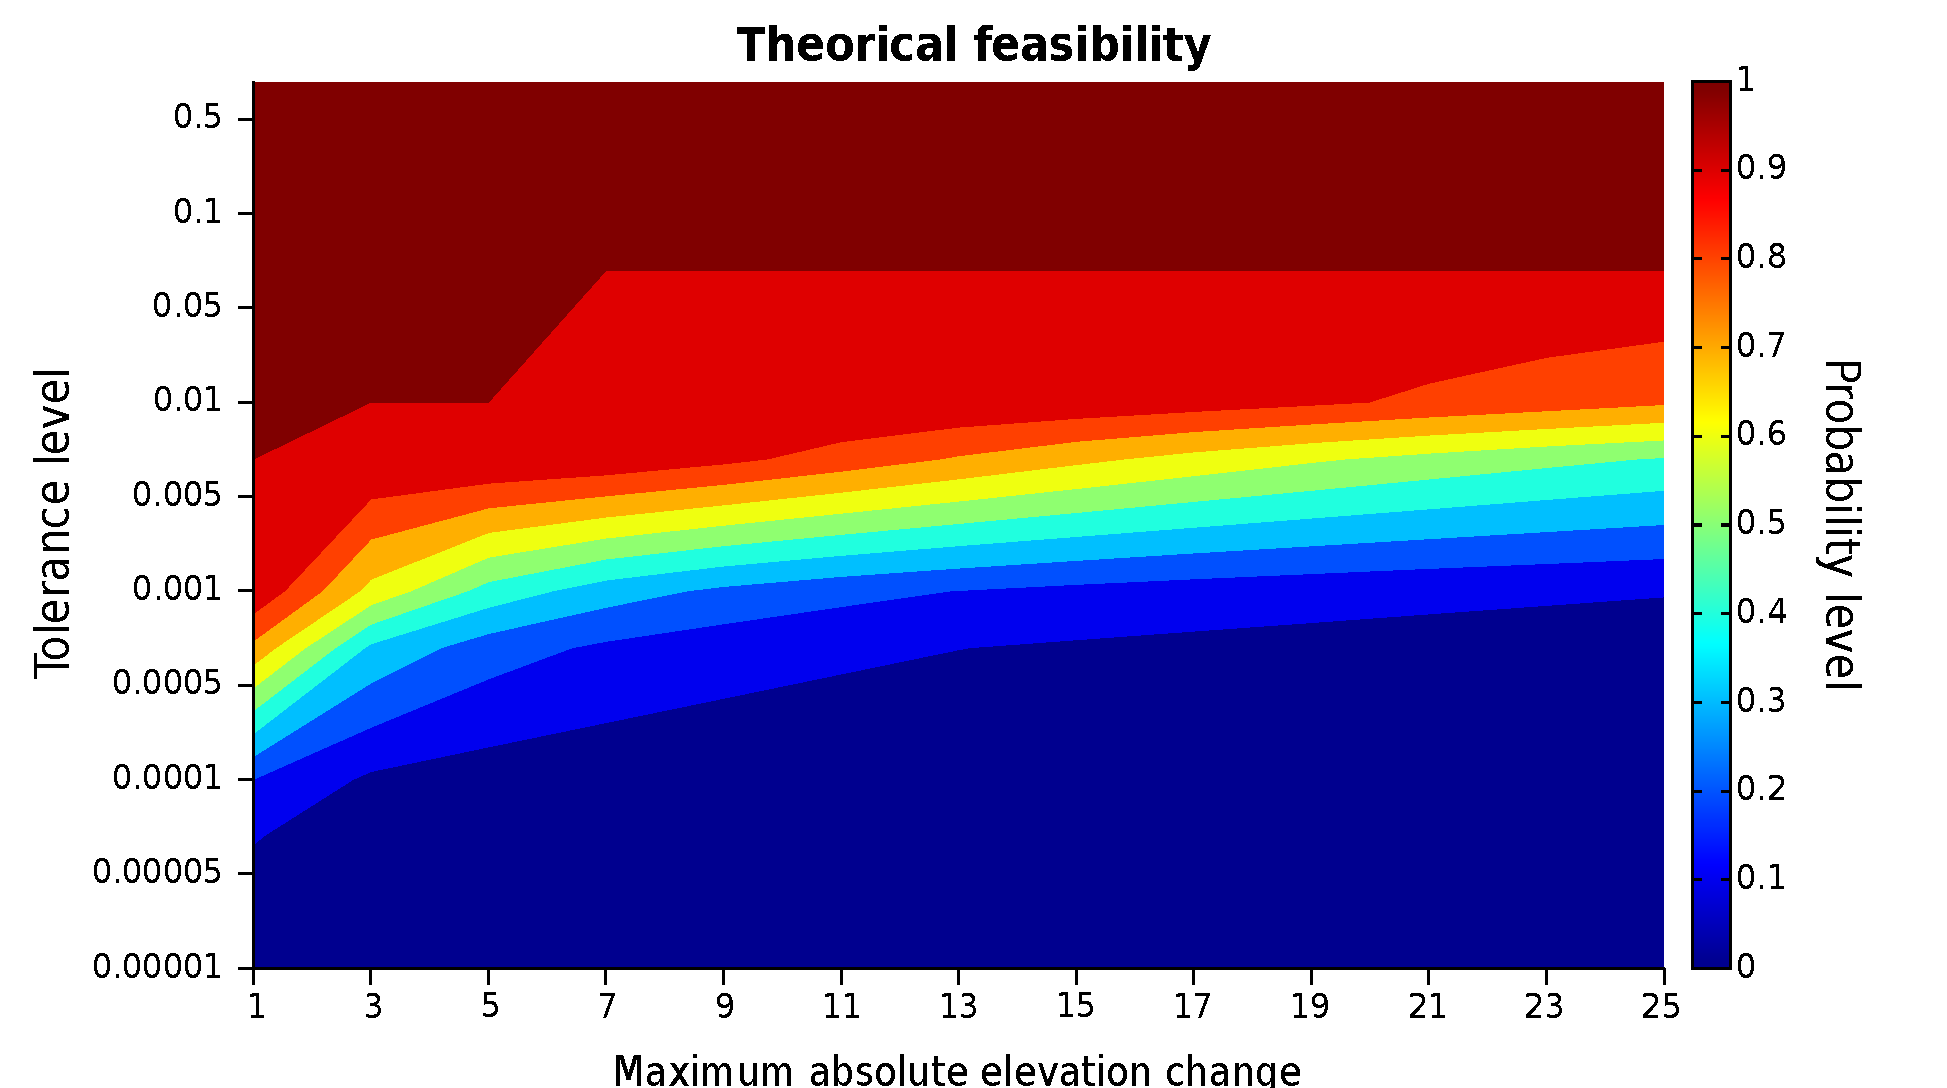
\includegraphics[width=\columnwidth]{Images/feasibilityNR51.pdf}  
\caption[Thing taken from our master thesis]{Thing taken from our master thesis whose meaning have been completely forgotten.}
\label{fig:massConstraintFeasibility}
\end{figure}

\begin{table}
\footnotesize
\centering
\begin{tabularx}{0.8\textwidth}{llrcl}
\toprule
\tableheadline{l}{Algorithm} &
\tableheadline{l}{Parameter} &
\tableheadlineMore{3}{c}{Suggested Values} \\
\midrule
\tablefirstcol{l}{Any}	& NFE	 		& $10\,000 $ 	& $ \div $ 	& $ 200\,000$ \\
				& Population Size 	&  $10 $ 		& $ \div $ 	& $ 1000$ \\
\midrule
\tablefirstcol{l}{GDE3} & DE step size 		& $0.0 $ 	& $\div $ 	& $ 1.0$ \\
				& Crossover rate 	& $0.0$ 	& $ \div $ 	& $ 1.0$ \\
\bottomrule
\end{tabularx}
\caption[Parameters needed for things]{Parameters needed for things that are not needed anymore themselves.}
\label{tab:MOEAandParameters}
\end{table}

\section{Contributing to this template}
Suggestion and improvements are welcome at \url{https://github.com/Lordmzn/ClassicThesis-at-DEIB} or via email at \url{emanuele.mason@polimi.it} or \url{andrea.cominola@polimi.it}.